\label{sec:CNN}
Convolutional Neural Networks (CNNs) are neural networks that predict the content of an input image by using assumptions about the local relationships between neighboring pixels. For this analysis, content prediction is simplified to a general classification of whether the image comes from a di-Higgs or QCD event. The fundamental elements of any convolutional network are convolutional layers and pooling layers. Convolutional layers use filters that perform linear combinations of neighboring pixels within the filter size, and pooling layers aggregate information by grouping neighboring pixels using either their maximum or average values. After some number of these layers, the output is flattened into a one-dimensional vector, and this flattened vector is pushed through a set of feed-forward layers in order to make a final output prediction. 

Many previous papers have explored the use of convolutional networks trained on low-level quantities (e.g. tracks and calorimeter deposits) for the purposes of object identification~\cite{Alison:2019kud} at colliders. This paper extends the application to event-level identification. Using low-level quantities removes the need to reconstruct higher-level objects like jets or jet pairs; only the detector-level measurements are required for image creation. The performance of four convolutional networks was studied in the context of di-Higgs identification. The first network used a 3-layer image composed of energy/momentum weighted tracks, electromagnetic calorimeter deposits, and hadronic calorimeter deposits. The second network used the same three layers but appended additional global event-level information to the flattened vector after image processing and before the fully connected layers. Figures~\ref{fig:cnn_nominal} and \ref{fig:cnn_hybrid} depict both network structures. The third and fourth networks followed the same pattern as the previous two but with the addition of two image layers corresponding to longitudinal and transverse impact parameter-weighted track information.

\begin{figure}[!h] 
\begin{center}
\includegraphics*[width=0.75\textwidth] {CNN/figures/nominalCNN.png}
\caption{Structure of the nominal convolutional neural network. The input images are fed through two convolutional layers and a single max-pooling layer before being flattened into a one-dimensional vector. The flattened vector is then fed through one fully connected layer, a batch normalization layer, and a final fully connected layer before a final prediction is made.}
  \label{fig:cnn_nominal}
\end{center}
\end{figure}

\begin{figure}[!h] 
\begin{center}
\includegraphics*[width=0.75\textwidth] {CNN/figures/hybridCNN.png}
\caption{Structure of the hybrid convolutional neural network. The input images are fed through two convolutional layers and a single max-pooling layer before being flattened into a one-dimensional vector. Scaled user-specified variables (e.g. $H_{T}$) are then concatenated with the flattened image vector. The concatenated vector is then fed through one fully connected layer, a batch normalization layer, and a final fully connected layer before a final prediction is made.}
  \label{fig:cnn_hybrid}
\end{center}
\end{figure}

In order to produce coherent images, the center of mass and the center of momentum for each event are calculated. All constituents are then boosted longitudinally into the center of mass of the event and rotated in phi to the center of momentum. After this pre-processing, each image layer corresponds to a 31x31 pixel grid centered on the total activity in the event. Figure~\ref{fig:cnn_avgImages} shows the average di-Higgs image layers (a--e) and the average QCD image layers (f--j). While the average image layers for each sample closely resemble one another, they do contain different information, and variations are visible.

Importantly, clear differences are observed between the average QCD images and the average di-Higgs images. Each half of the di-Higgs image (split across $\phi$ = 0) is arranged in a roughly circular, isotropic shape due to the spin-0 nature of the Higgs. The QCD images appear balanced because of the effect of the pre-processing, but no similar circular structure is produced. Additionally, the variance of pixel intensities in di-Higgs images is much smaller than the variance in QCD images due to the more balanced kinematics of Higgs pair production compared to QCD processes.

\begin{figure}[!ht] 
\begin{center}
  \subfloat[]{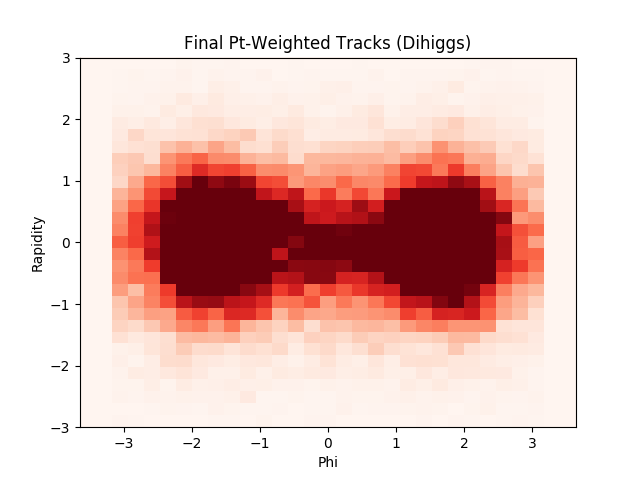
\includegraphics[width = 2in]{CNN/figures/images/hh/Tracks_Dihiggs_Final_Pt-Weighted}} 
  \subfloat[]{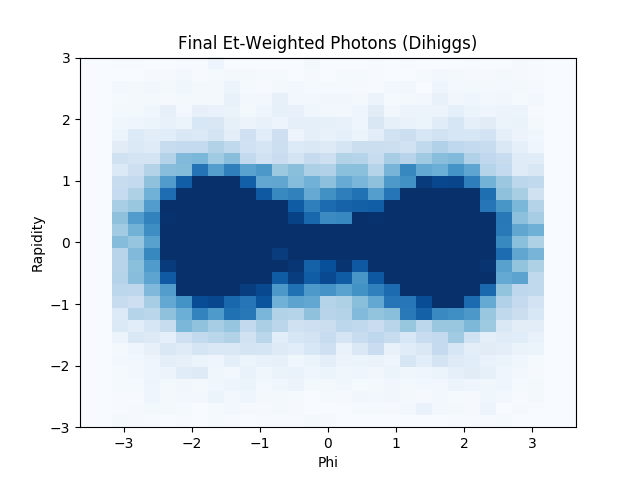
\includegraphics[width = 2in]{CNN/figures/images/hh/Photons_Dihiggs_Final_Et-Weighted}}
  \subfloat[]{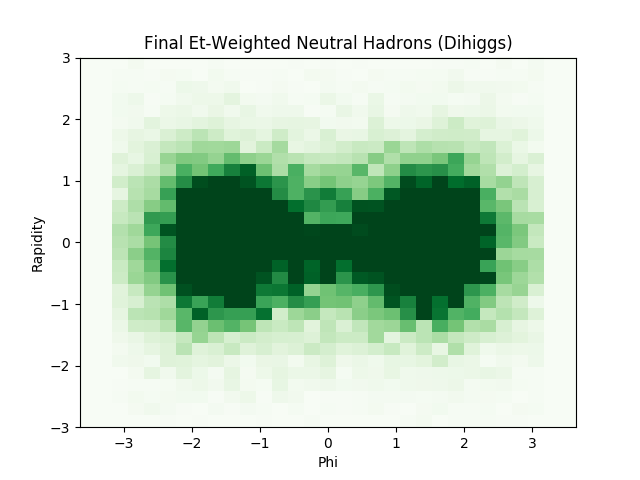
\includegraphics[width = 2in]{CNN/figures/images/hh/NeutralHadrons_Dihiggs_Final_Et-Weighted}} \\
  \subfloat[]{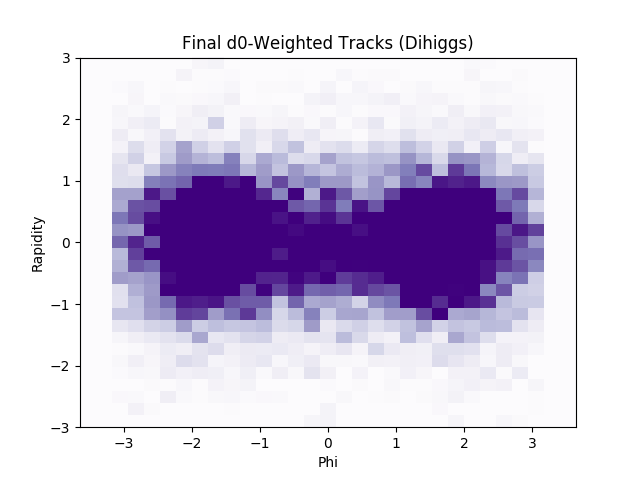
\includegraphics[width = 2in]{CNN/figures/images/hh/Tracks_Dihiggs_Final_d0-Weighted}} 
  \subfloat[]{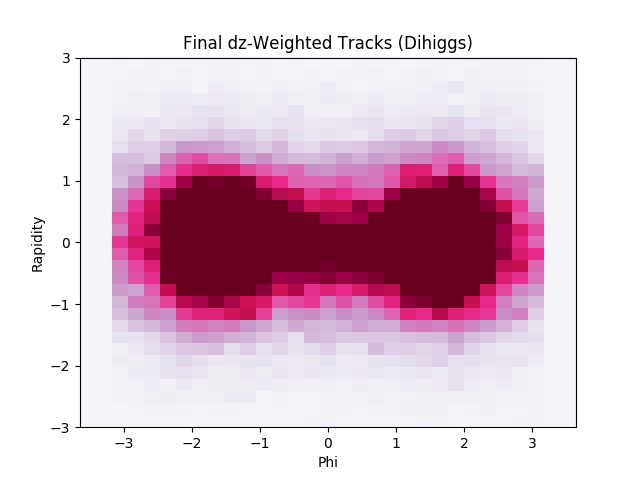
\includegraphics[width = 2in]{CNN/figures/images/hh/Tracks_Dihiggs_Final_dz-Weighted}} \\
  \subfloat[]{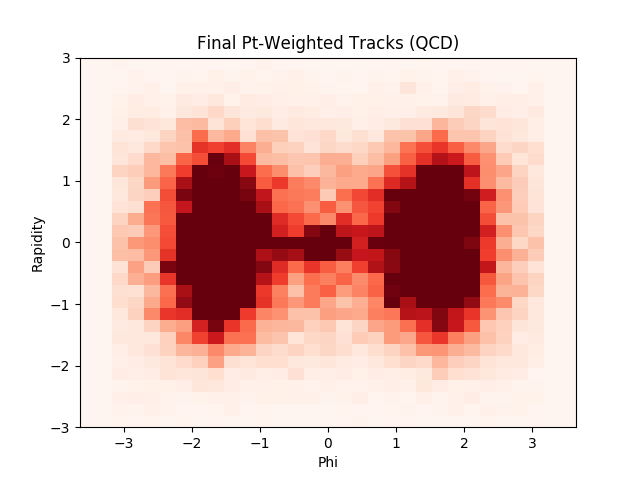
\includegraphics[width = 2in]{CNN/figures/images/qcd/Tracks_QCD_Final_Pt-Weighted}} 
  \subfloat[]{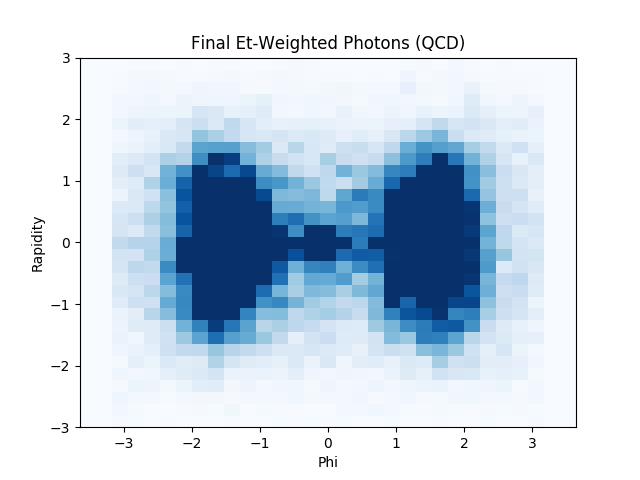
\includegraphics[width = 2in]{CNN/figures/images/qcd/Photons_QCD_Final_Et-Weighted}}
  \subfloat[]{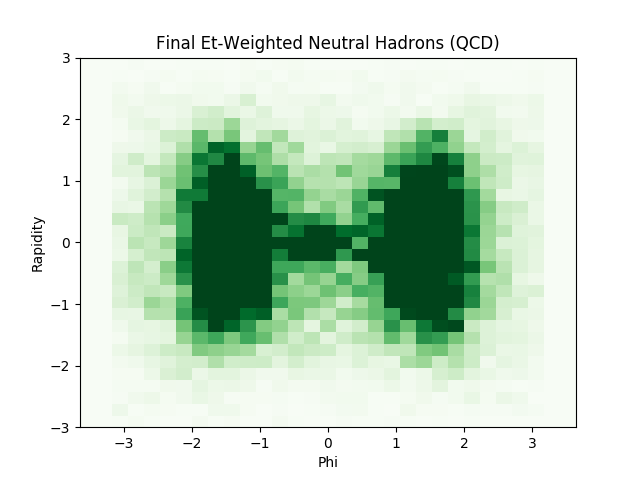
\includegraphics[width = 2in]{CNN/figures/images/qcd/NeutralHadrons_QCD_Final_Et-Weighted}} \\
  \subfloat[]{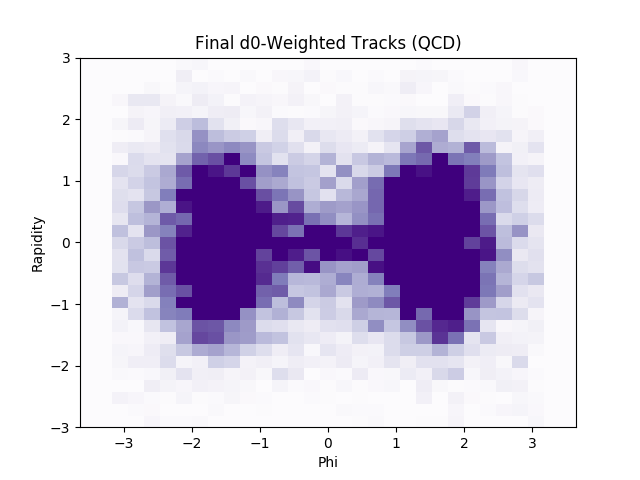
\includegraphics[width = 2in]{CNN/figures/images/qcd/Tracks_QCD_Final_d0-Weighted}} 
  \subfloat[]{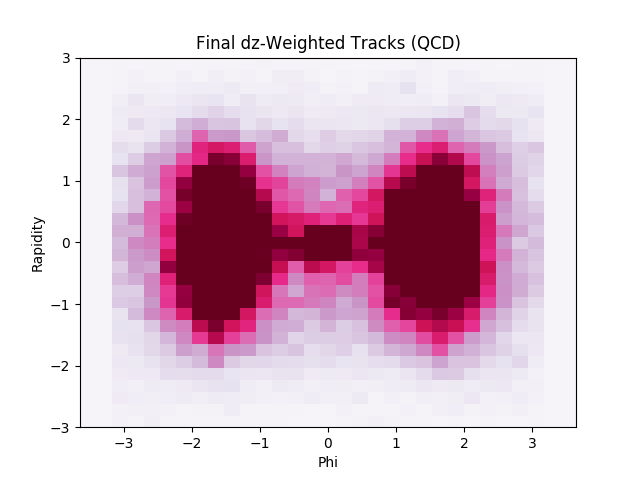
\includegraphics[width = 2in]{CNN/figures/images/qcd/Tracks_QCD_Final_dz-Weighted}} 
\caption{Average image layers for di-Higgs (a--e) and QCD (f--j) decays. Sub-figures (a) and (f) show $p_{\textrm{T}}$-weighted tracks, (b) and (g) show $E_{\textrm{T}}$-weighted ECAL deposits, (c) and (h) show $E_{\textrm{T}}$-weighted HCAL deposits, (d) and (i) show transverse impact parameter-weighted tracks, (e) and (j) show longitudinal impact parameter-weighted tracks.} %The differences between di-Higgs and QCD layers are apparent.}
\end{center}
\label{fig:cnn_avgImages}
\end{figure}

%\begin{figure}[!h] 
%\begin{center}
%  \subfloat[]{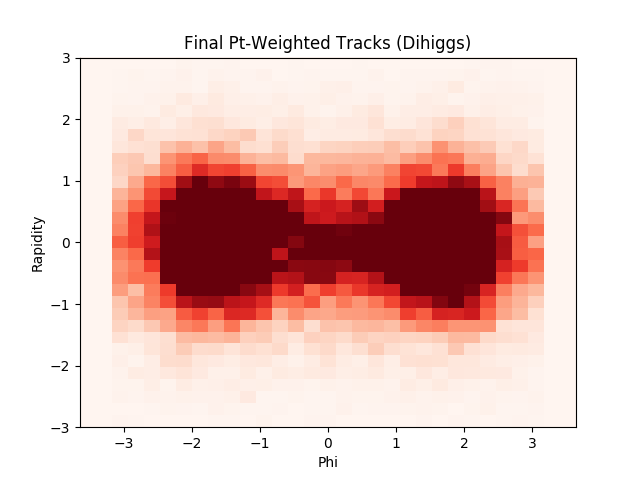
\includegraphics[width = 2in]{CNN/figures/images/hh/Tracks_Dihiggs_Final_Pt-Weighted}} 
%  \subfloat[]{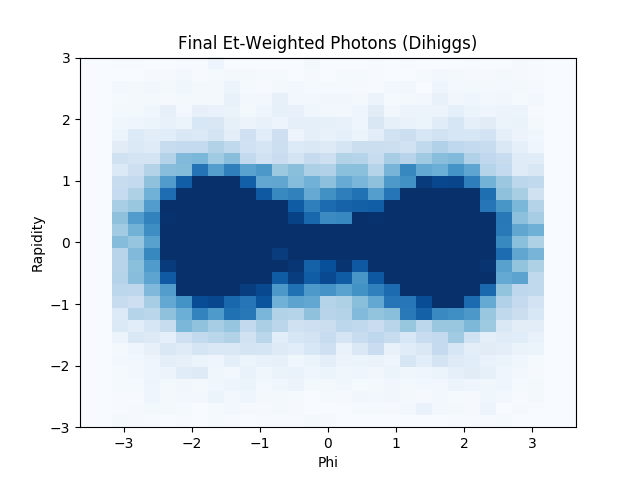
\includegraphics[width = 2in]{CNN/figures/images/hh/Photons_Dihiggs_Final_Et-Weighted}}
%  \subfloat[]{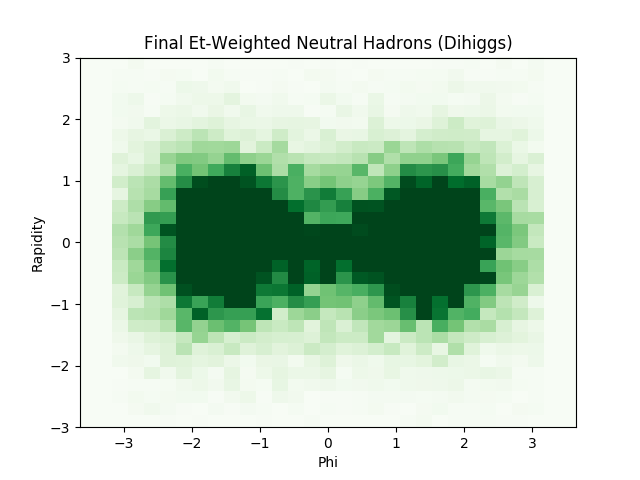
\includegraphics[width = 2in]{CNN/figures/images/hh/NeutralHadrons_Dihiggs_Final_Et-Weighted}} \\
%  \subfloat[]{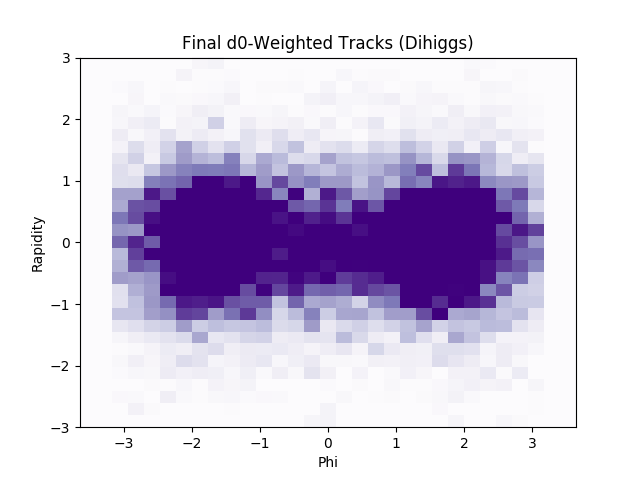
\includegraphics[width = 2in]{CNN/figures/images/hh/Tracks_Dihiggs_Final_d0-Weighted}} 
%  \subfloat[]{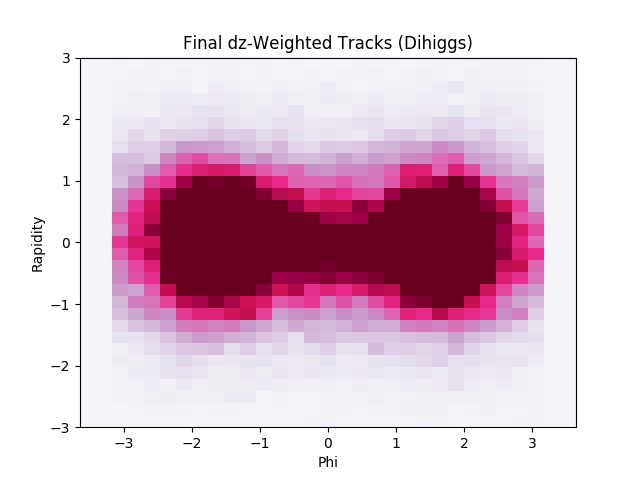
\includegraphics[width = 2in]{CNN/figures/images/hh/Tracks_Dihiggs_Final_dz-Weighted}} 
%\caption{Average di-Higgs image showing (a) $p_{\textrm{T}}$-weighted tracks, (b) $E_{\textrm{T}}$-weighted ECAL deposits, (c) $E_{\textrm{T}}$-weighted HCAL deposits, (d) transverse impact parameter-weighted tracks, (e) longitudinal impact parameter-weighted tracks.}
%\end{center}
%\label{fig:cnn_avgDihiggs}
%\end{figure}

As shown in Figures~\ref{fig:cnn_nominal} and \ref{fig:cnn_hybrid}, the CNN network structure uses two sequential 2D convolutional layers each with 16 3x3 filters, one max-pooling layer with a 2x2 window, a flattening of the outputs, two 64-node fully connected hidden layers, and one output layer for making the final prediction. As previously described, two of the networks append additional high level variables (scalar sum of transverse hadronic energy, number of jets, and number of $b$-tags) after the flattening and before the image information is fed through the fully connected layers. The optimal significance for each network is shown in Table~\ref{tab:cnnResults}. The best results were obtained using the 5-color network with additional high-level inputs, and the final predictions for this configuration are shown in Figure~\ref{fig:cnn_preds}. A best significance of 2.86$\pm$0.03 was found for a prediction cut $>$ 0.94 with a signal yield of $1.00\pm 0.05$ $\cdot$ $10^4$ events and a background yield of $1.32\pm 0.01$ $\cdot$ $10^7$ events.

\begin{table}[h!]
\label{tab:cnnResults}
  \begin{center}
    \begin{tabular}{|l|c|c|} % <-- Alignments: 1st column left, 2nd middle and 3rd right, with vertical lines in between
      \hline\hline
      \textbf{Method} & Best $\sigma$ & AUC \\
      \hline
      Tracks+HCAL+ECAL & 1.77 $\pm$ 0.01 & 0.818 \\
      Tracks+HCAL+ECAL + high-level & 2.12 $\pm$ 0.01 & 0.846 \\
      Tracks+HCAL+ECAL+D0+DZ & 2.45 $\pm$ 0.02 & 0.863 \\
      Tracks+HCAL+ECAL+D0+DZ + high-level & 2.86 $\pm$ 0.03 & 0.882 \\

      \hline\hline
    \end{tabular}
    \caption{Normalized to full HL-LHC dataset of 3000 fb$^{-1}$}
  \end{center}
\end{table}


\begin{figure}[!h] 
\begin{center}
  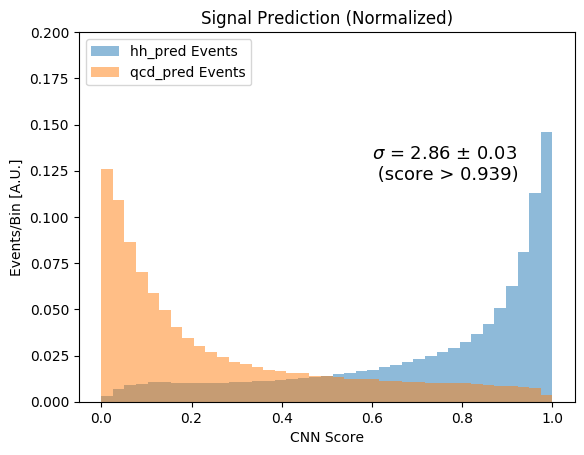
\includegraphics[width = 3in]{CNN/figures/5color_0PU_pix31_addHT-nJets-nBTags_2Conv16-16_one2DPool_EqualSamples/signal_CNNScore_norm}
  %\subfloat[]{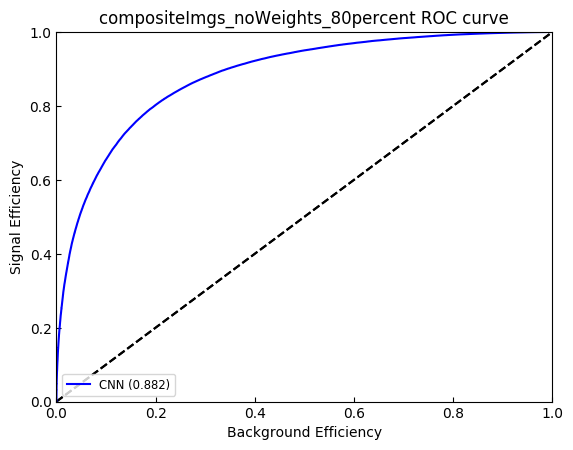
\includegraphics[width = 3in]{CNN/figures/5color_0PU_pix31_addHT-nJets-nBTags_2Conv16-16_one2DPool_EqualSamples/compositeImgs_noWeights_80percent_ROC}}\\
\caption{Signal prediction for the 5-color convolutional network with additional high-level inputs. The total area of the signal and background predictions are normalized to unity for easier shape comparison.}
\end{center}
\label{fig:cnn_preds}
\end{figure}

